\chapter{Pixel-based Analysis}

\section{Diurnal cycles}
\label{sec:diurnal_cycle}
In the following, we consider the total fraction of pixels that satisfy certain conditions. This fraction is also called coverage in the following. Two different variables are analysed:
\begin{enumerate}
\item The CI product data have been masked under the condition that each CI pixel is greater than or equal to a certain, selected CI threshold. This results in masks that select CI with probability equal to or greater than a certain value, e.g. all CI pixels are selected with a probability larger than 50\%, that combines the intervals 50-75\% and $>75$\%. In other words, the provided CI levels have been combined to cumulative CI probabilities for further analysis with the following meaning:
\begin{itemize}
    \item $\textrm{Prob}_{CI}\ge 0\%$  $\equiv$  CI indicator interval $]0, 100] \%$
    \item $\textrm{Prob}_{CI}\ge 25\%$  $\equiv$  CI indicator interval $]25, 100] \%$, etc.
\end{itemize}
\item Radar RX data are masked under the condition that radar reflectivities are greater than a threshold of 35 dBZ. The fractional coverage is called $f_{>35 \mathrm{dBZ}}$.
\end{enumerate}

The fractions of pixels that satisfy the conditions mentioned above are calculated for each time slot and date separately. The results are shown in Figs.~\ref{fig:dc20100523} to \ref{fig:dc20130620}. Looking at the diurnal cycle of the fractional coverage of low probability CI events (with $>0\%$ and $>25\%$), one can not recognise any reasonable connection to the diurnal cycle of higher probability CI events (with $>50\%$ and $>75\%$). The two low probability curves are in general very close together. Furthermore, there is more than one order of magnitude difference between the low and high probability CI counts. This means that the low probability CI categories are not well calibrated, and might be not reasonably connected to precipitation formation probability at all. Therefore, to our opinion, the low probability CI categories are likely to be useless.

In the next, we focus on the higher probability CI events (with $>50\%$ and $>75\%$). They cover only a very small fraction and therefore represent only a small number of events. Thus, conclusions based on the six case days are very likely to be statistically poorly significant. By inspection 
of Figs.~\ref{fig:dc20100523} to \ref{fig:dc20130620}, it can be seen that both categories show the main activity between noon and early evening. This is also the time period when the relative fraction of radar reflectivities $>35$ dBZ is increasing (except for the 28 June 2010 where no significant heavy precipitation was recorded) and where the temporal differences in $f_{>35\mathrm{dBZ}}$ are positive. This, of course, only gives a very general indication of an increased precipitation formation activity that comes along with an increase number of issued CI detections.

\begin{figure}
\centering
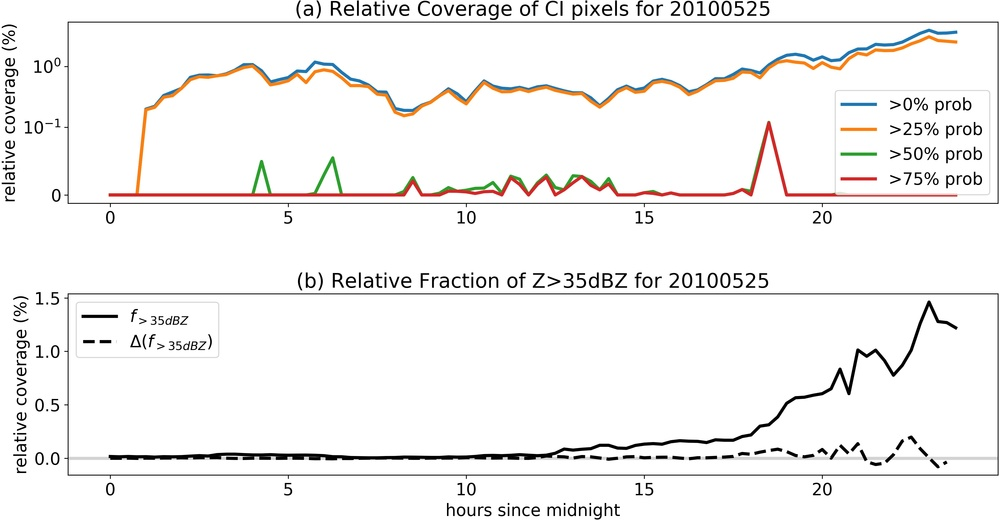
\includegraphics[width=\textwidth]{Grafiken/Abbildungen/diurnal_cycle_20100525.jpg}
\caption{Diurnal cycles of the fractional coverage of (a) CI pixels with a certain probability level (coloured lines) and (b) RX radar reflectivity pixels above 35 dBZ (black solid line) for the 25 May 2010. Please note that the upper part of the y-axis in panel a is logarithmic. The temporal change of $f_{>35\mathrm{dBZ}}$ is shown in panel b with a dashed black line. The curve has been smoothed with a running mean with a window of 3.}
\label{fig:dc20100523}
\end{figure}
%%%%%%%%%%%%%%%%%%%%%%%%%%%%%%%%%%%%%%%%%%%%%
\begin{figure}
\centering
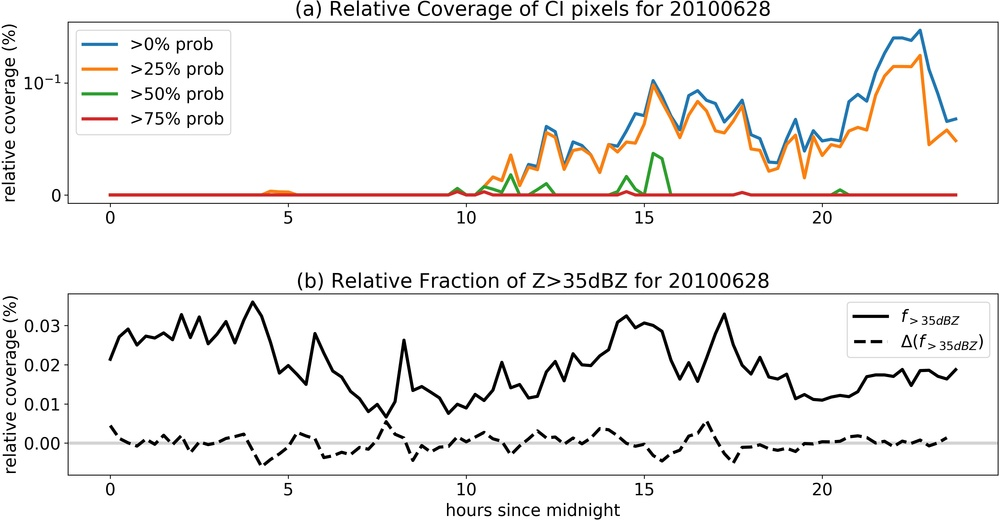
\includegraphics[width=\textwidth]{Grafiken/Abbildungen/diurnal_cycle_20100628.jpg}
\caption{Same as Fig.~\ref{fig:dc20100523}, but for the 28 June 2010.}
\label{fig:dc20100628}
\end{figure}
%%%%%%%%%%%%%%%%%%%%%%%%%%%%%%%%%%%%%%%%%%%%%
\begin{figure}
\centering
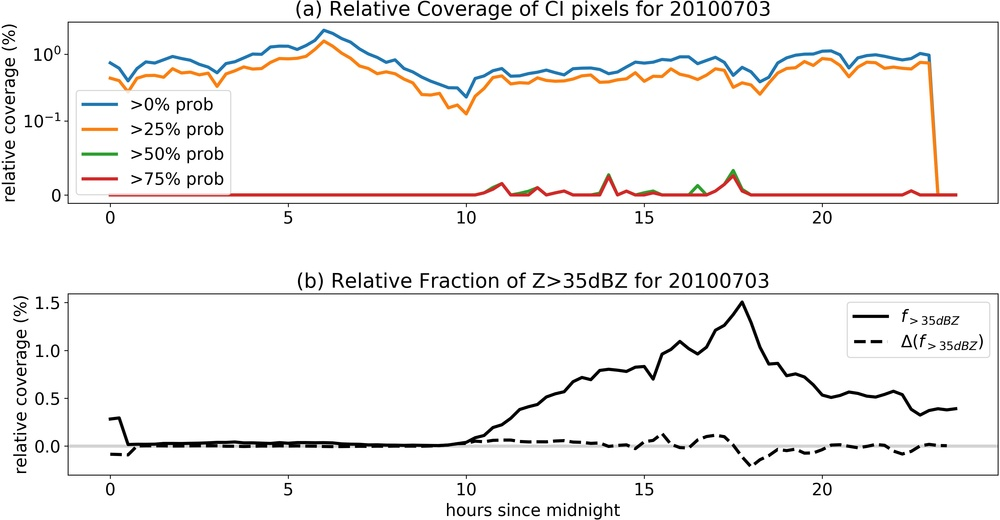
\includegraphics[width=\textwidth]{Grafiken/Abbildungen/diurnal_cycle_20100703.jpg}
\caption{Same as Fig.~\ref{fig:dc20100523}, but for the 3 July 2010.}
\label{fig:dc20100703}
\end{figure}
%%%%%%%%%%%%%%%%%%%%%%%%%%%%%%%%%%%%%%%%%%%%%
\begin{figure}
\centering
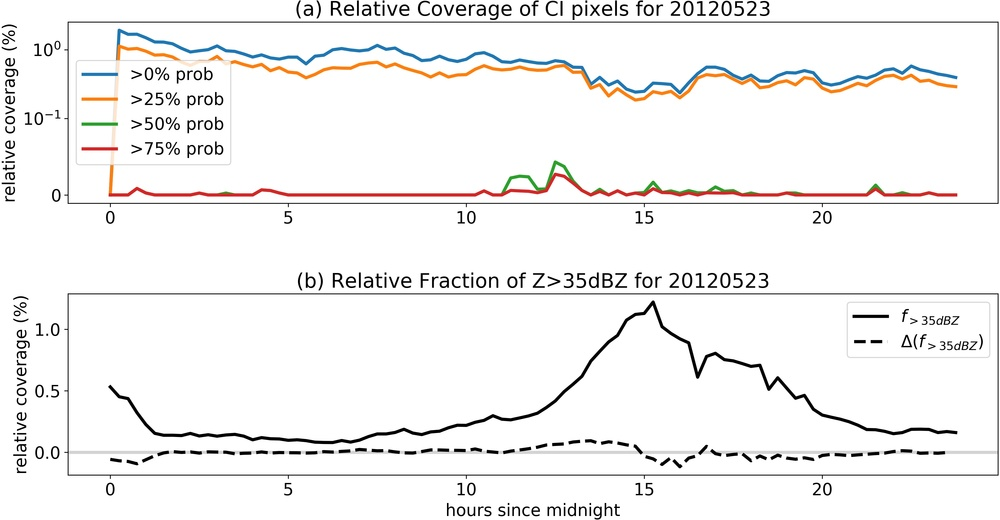
\includegraphics[width=\textwidth]{Grafiken/Abbildungen/diurnal_cycle_20120523.jpg}
\caption{Same as Fig.~\ref{fig:dc20100523}, but for the 23 May 2012.}
\label{fig:dc20120523}
\end{figure}
%%%%%%%%%%%%%%%%%%%%%%%%%%%%%%%%%%%%%%%%%%%%%
\begin{figure}
\centering
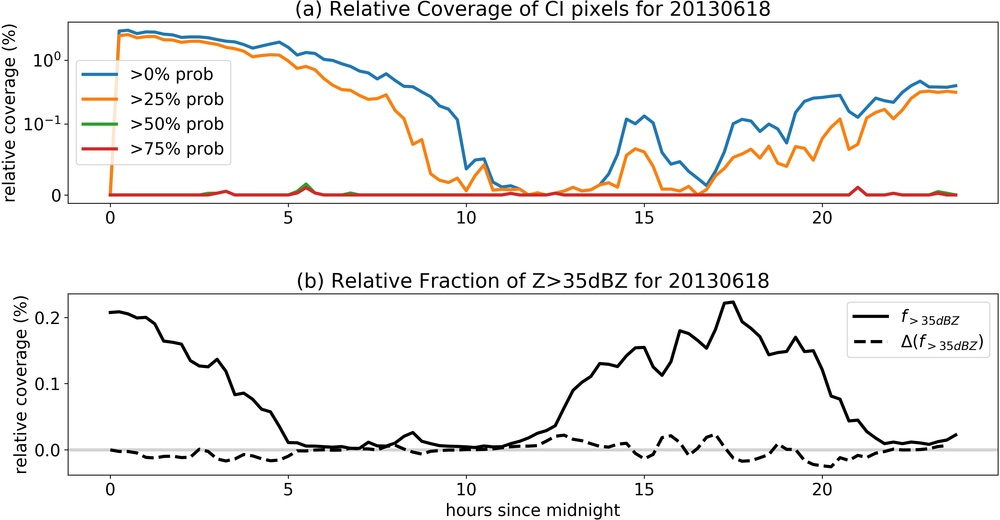
\includegraphics[width=\textwidth]{Grafiken/Abbildungen/diurnal_cycle_20130618.jpg}
\caption{Same as Fig.~\ref{fig:dc20100523}, but for the 18 June 2013.}
\label{fig:dc20130618}
\end{figure}
%%%%%%%%%%%%%%%%%%%%%%%%%%%%%%%%%%%%%%%%%%%%%
\begin{figure}
\centering
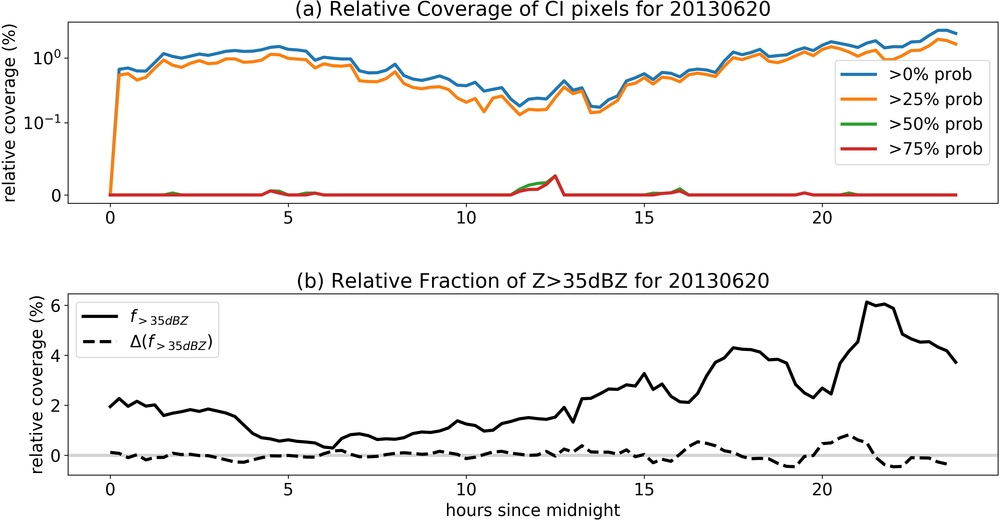
\includegraphics[width=\textwidth]{Grafiken/Abbildungen/diurnal_cycle_20130620.jpg}
\caption{Same as Fig.~\ref{fig:dc20100523}, but for the 20 June 2013.}
\label{fig:dc20130620}
\end{figure}

\section{Connection between CI detections and already existing precipitation}
From the movies \footnote{hosted at https://owncloud.gwdg.de/index.php/s/nwiyGQBFbN1FaH9, visited at 8 Nov 2018} generated by TROPOS for the case days which combine the CI product with radar data, one could get the impression that a significant fraction of CI detections occur in regions where radar reflectivities are already large. Depending on the interpretation of the CI product, a CI detection within or close to radar reflectivity contours $>35$ dBZ would be a false detection, as we would require that the CI detection marks a newly  developing precipitation cell and not an already existing one. In the above argument, we already used the word "cell". From a realistic precipitation field, it is often not clear what a "cell" is and how newly formed precipitation can be objectively detected. 

As noted above, the fraction of low probability CI detections is not connected to their higher probability counterpart and also does not follow the diurnal cycle in heavy precipitation changes. It is indeed the low probability CI field that has significant overlap with high radar reflectivities (not shown) and which introduces this above mentioned impression when viewing the movies. 

In contrast, the higher probability CI detections, here the $>50\%$-category was chosen, has much smaller overlap to the radar $>35$\,dBZ field. Results of an analysis are shown in Fig.~\ref{fig:overlap_CI50-RX}. For the analysis, the parallax transformation was applied first to the CI product data. Subsequently, masks have been generated from the parallax-corrected CI data selecting a certain probability category. 

Thereafter, histograms of the absolute frequency of the radar reflectivities within the selected CI areas have been computed. The results in Fig.~16 show that most of the CI detections appear in areas where no significant precipitation is present. Maximum overlap with $>35$\,dBZ appears with 7.1\% for 3 July 2010 and with 4.1\% for 18 June 2013. The low fractional overlap between CI areas and high precipitation areas is desirable as CI detections should indicate newly developing precipitation cells. Therefore, the small overlap on the order of a few percent for the higher probability CI detection is a very promising result.

\begin{figure}
\centering
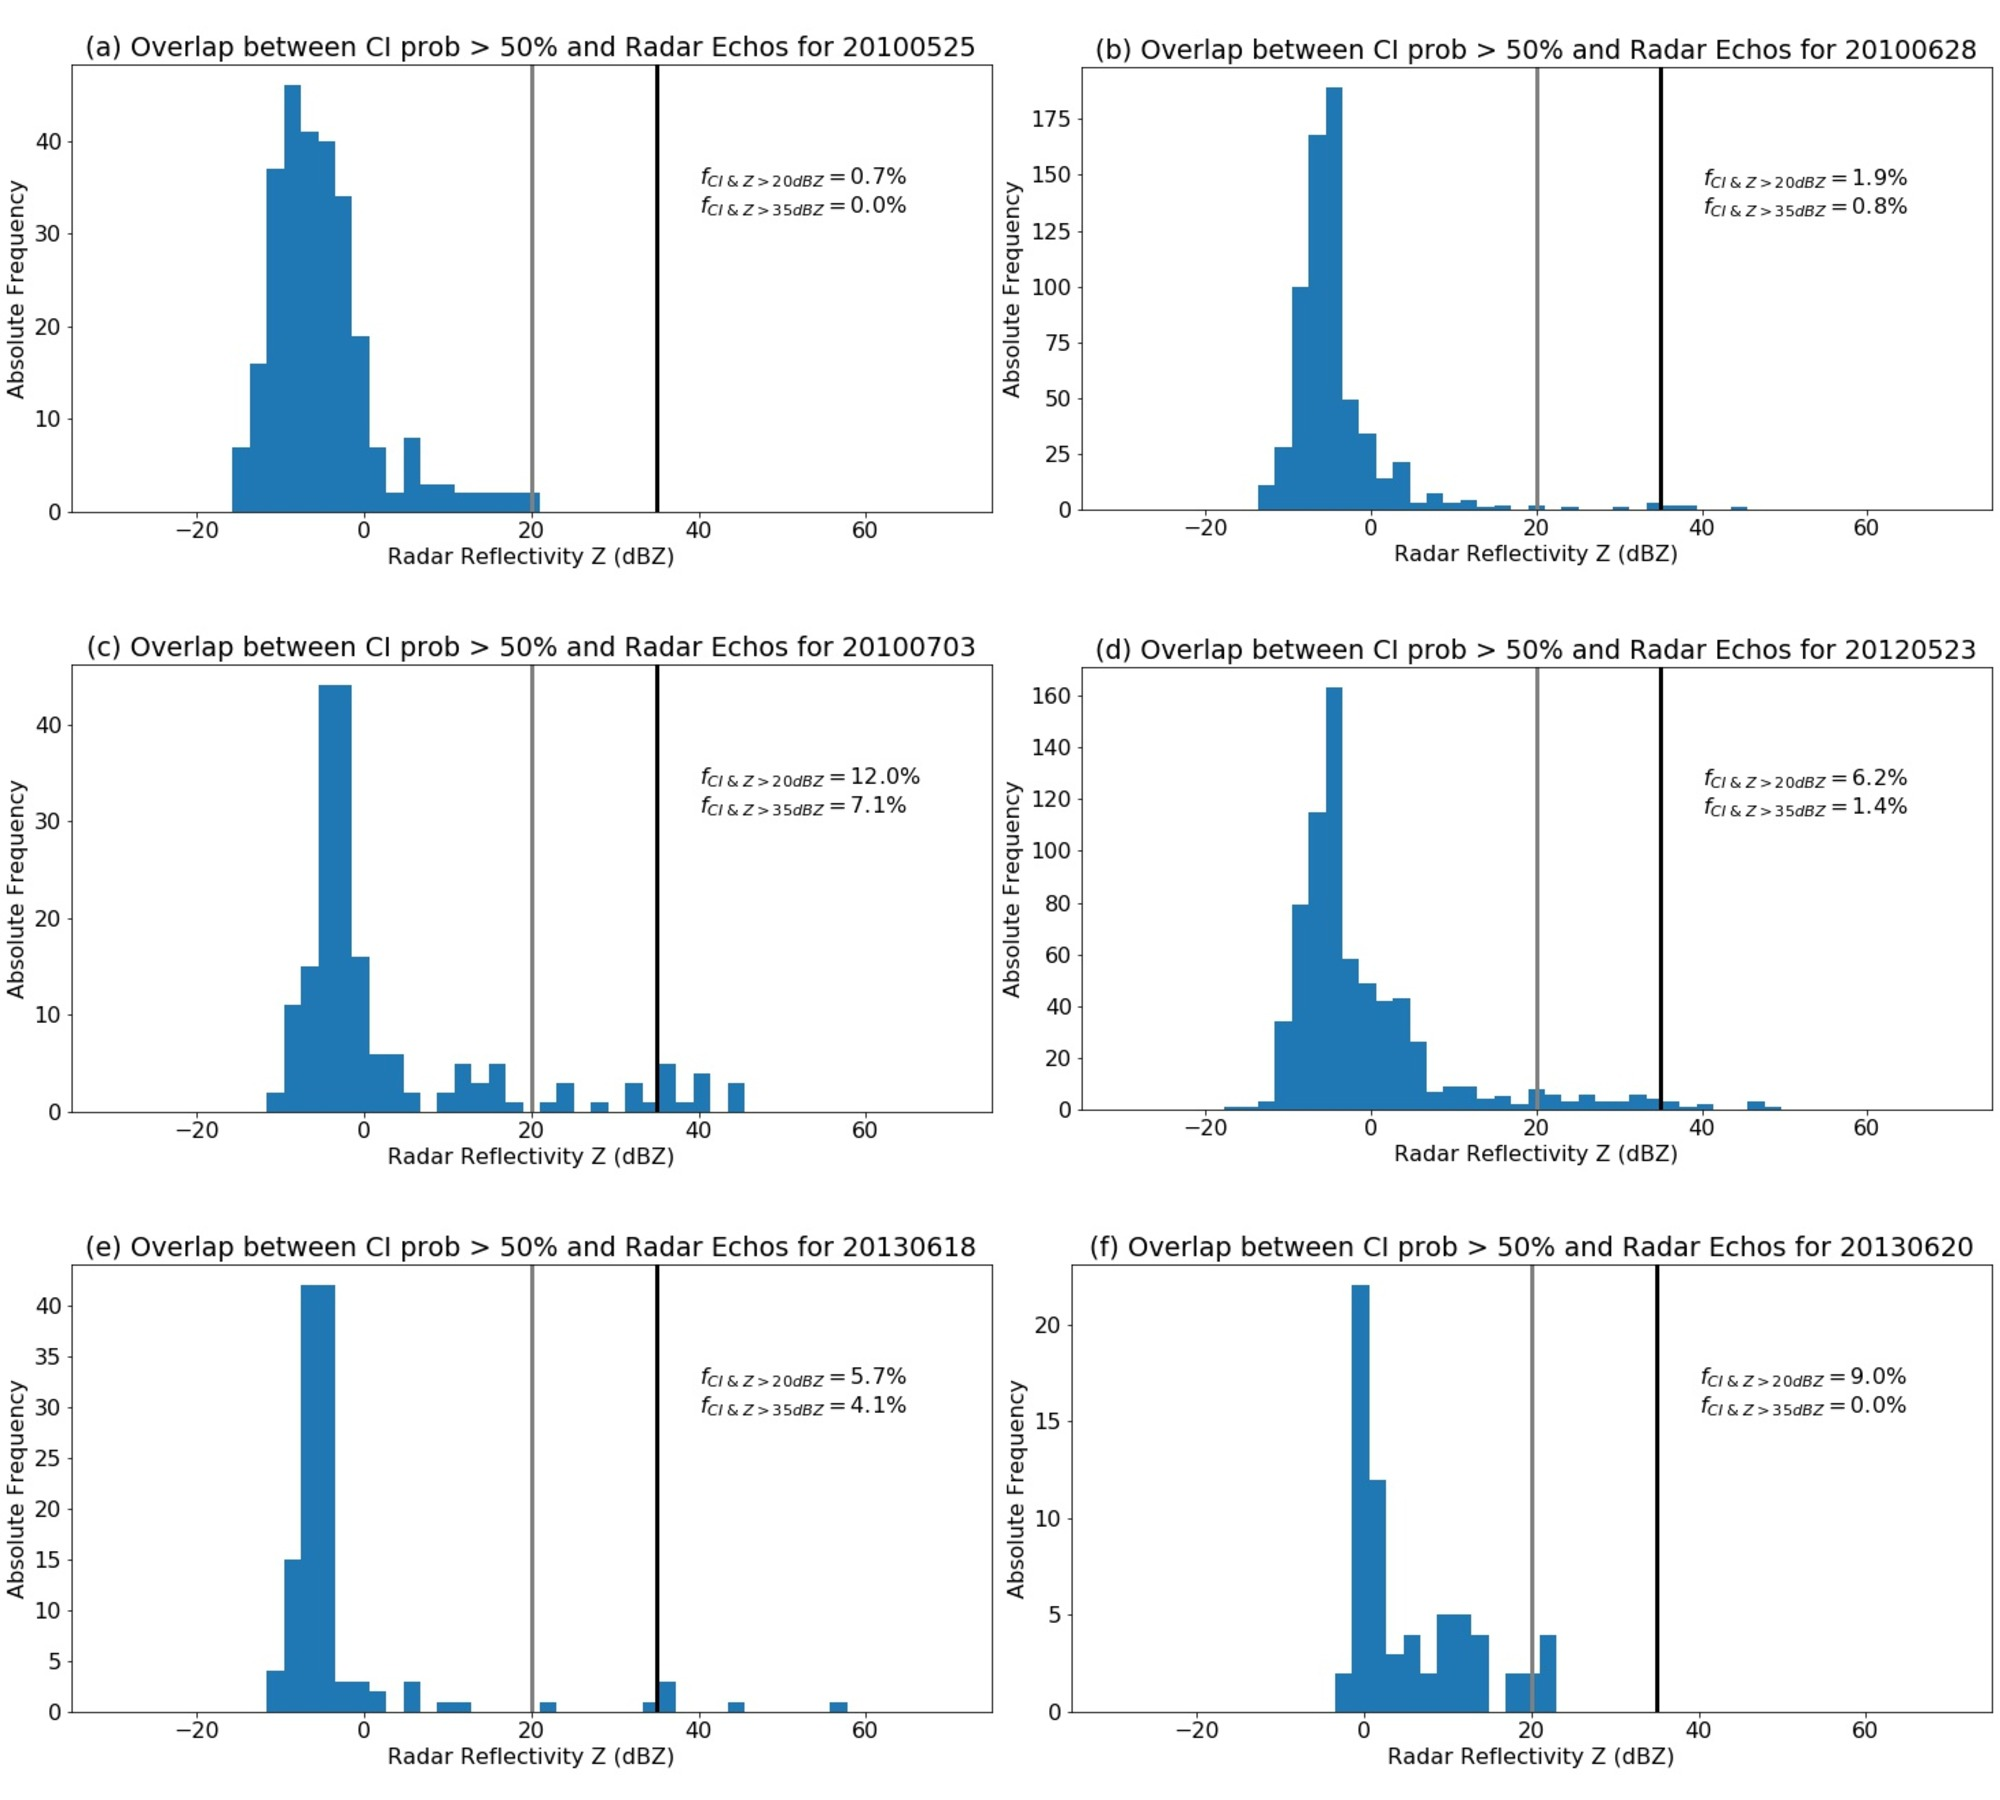
\includegraphics[width=\textwidth]{Grafiken/Abbildungen/overlap_CI50_RX.jpg}
\caption{Absolute Frequencies of radar reflectivities for CI detections with probability greater than 50\% for all six case days in chronological order (a) to (f). Two thresholds at 20 and 35 dBZ are marked with vertical lines.}
\label{fig:overlap_CI50-RX}
\end{figure}

A second analysis is again devoted to the question if CI detections occur in places where radar reflectivities are already large. Therefore, we measure the Euclidean distance between each of the CI pixels to the closest radar 35 dBZ contour. We excluded radar-derived objects smaller than 16 pixels to decrease sensitivity to false echoes and artifacts in the radar data. The absolute frequencies of distance counts are shown in Fig.~\ref{fig:distance_CI50-RX35}. It is hard to select a threshold distance at which a CI detection is considered to be too close to an existing precipitation event. If we select 15 km minimum distance, which is the buffer radius chosen for the radar object analysis, we see that in most of the cases only a small fraction of CI detection is closer than this distance. One exception is the distance statistic for the 23 May 2012. In this case, 22\% of the CI detections are very close to already existing precipitation. Please note that the distance analysis is very dependent on the CI object sizes and the general spatial distribution of the precipitation field.

\begin{figure}
\centering
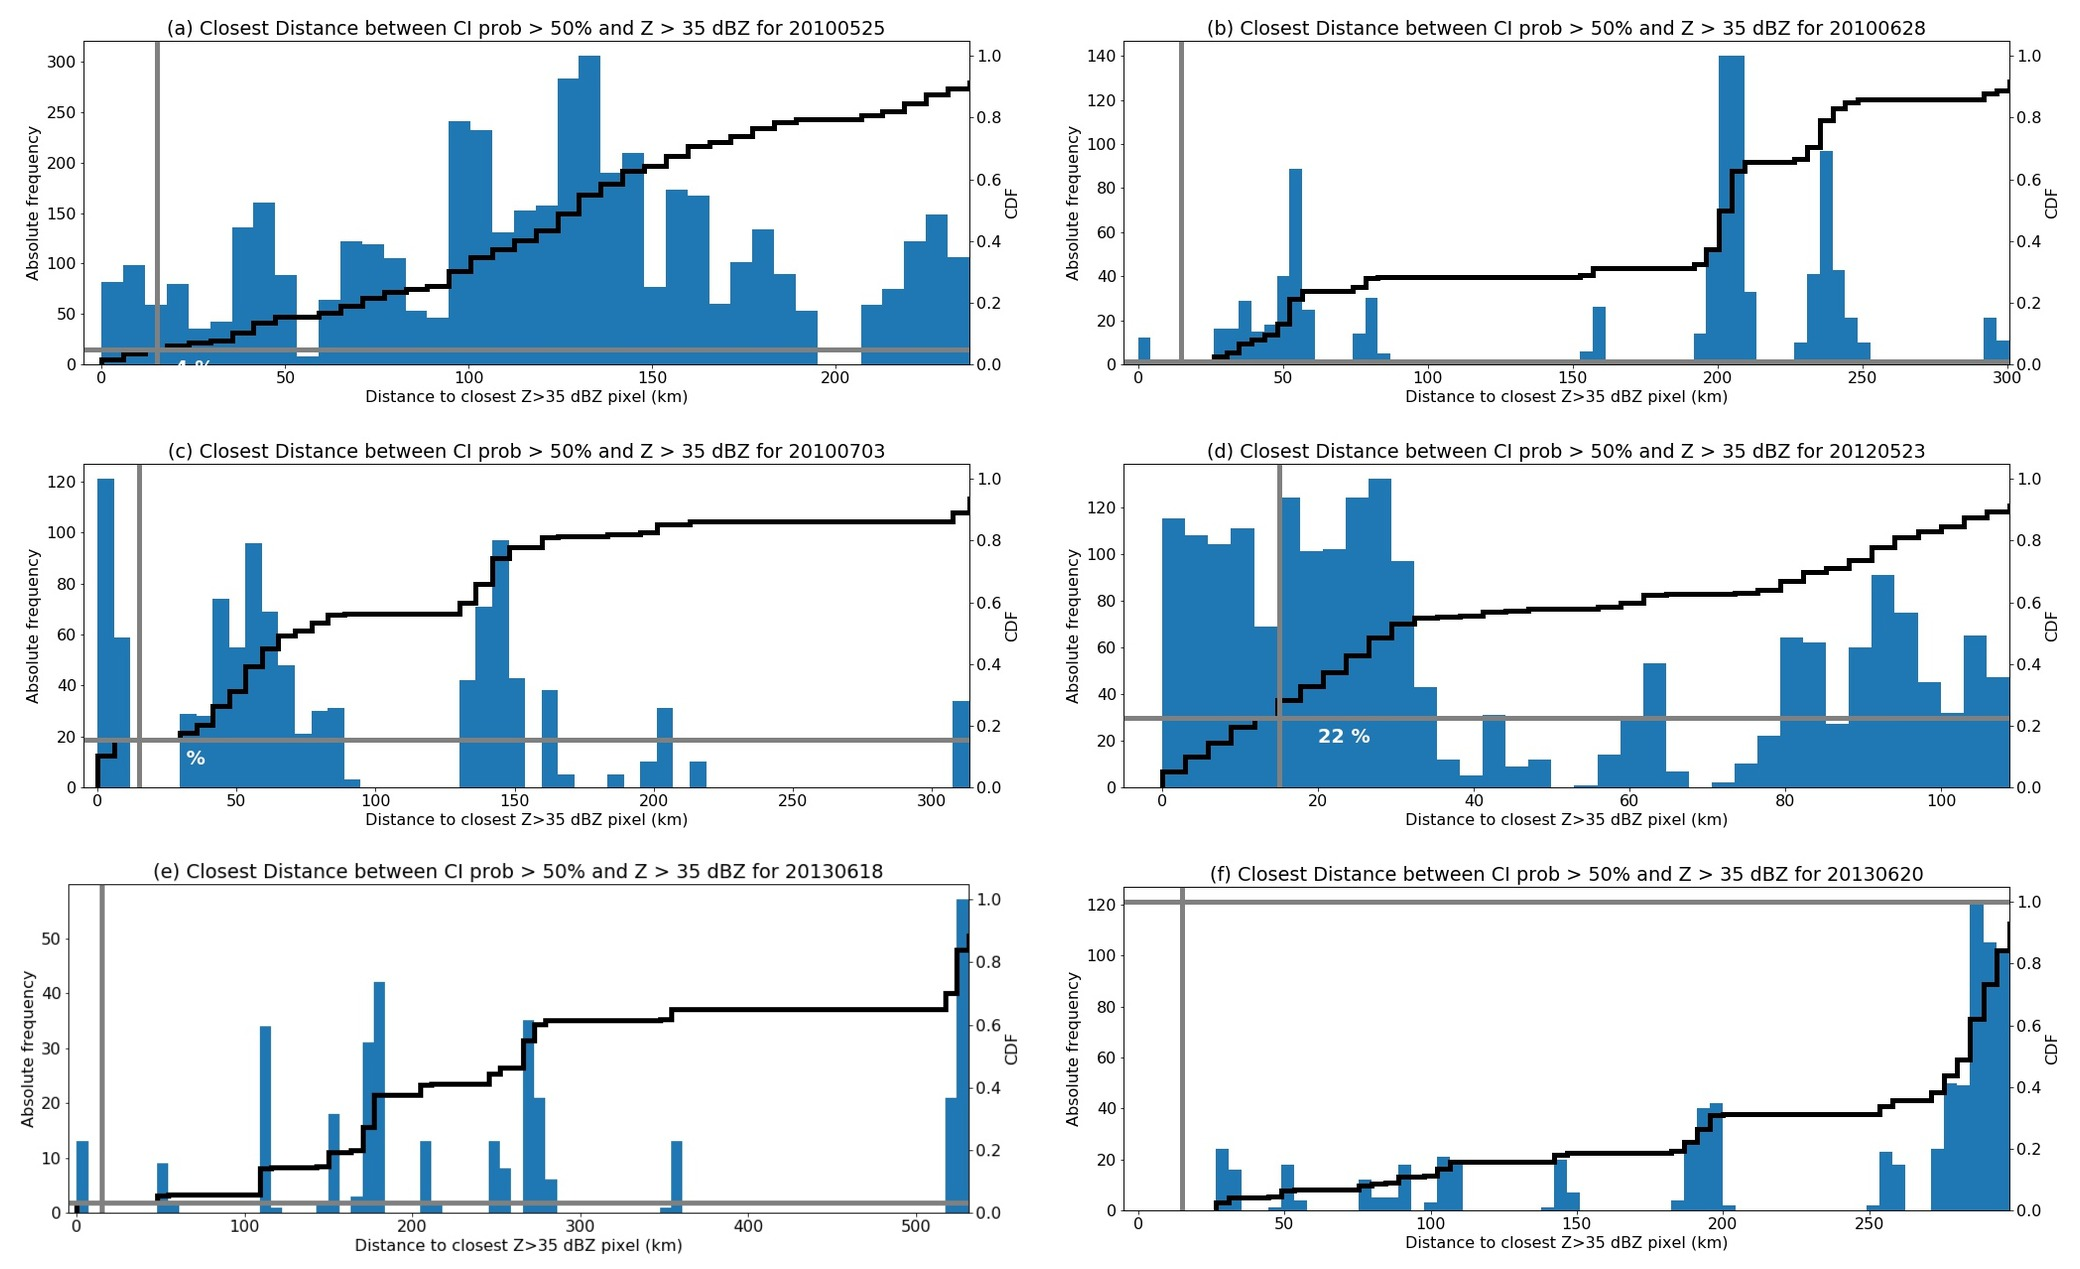
\includegraphics[width=\textwidth]{Grafiken/Abbildungen/distance_CI50_RX35.jpg}
\caption{Absolute Frequencies of distances to the closest 35 dBZ contour for CI detections with probability greater than 50\% (On each left y-axis, blue bars) for all six case days in chronological order (a) to (f). In addition, the panels shows the cumulative probability to have a 35 dBZ reflectivity contour closer than a certain distance (black solid lines).}
\label{fig:distance_CI50-RX35}
\end{figure}

\section{Temporal persistence of CI detections}
Also inspired by the provided cloud and precipitation movies, the question arises how long CI detections do last. Persistent CI detection indicate places where the probability for precipitation formation remains high. This is not  a problem on its own, and persistent CIs do not have to be false detections. However, if CI is issued with high probability at a certain place, one would expect for a high-quality detection, that precipitation will form within 30~min. A persistent CI that lasts more than 30\,min would not be appropriate in this case.

For the pixel-based analysis, we only consider the Eulerian perspective, i.e. we do not correct for the motion of clouds and their associated CI detections. As a first similar measure, we analyse spatial auto-correlation functions (see Fig.~\ref{fig:decorr_analysis}). CI fields with a small but fixed time lag have been compared with the help of linear pattern correlation coefficients. The resulting curve describes the de-correlation behaviour of the CI fields. Largest e-folding times with more than 75\,min are obtained for the 23 May 2012. For this case, long-lived cloud structures with a rather slow movement seem to imprint on the CI detections. For most of the other cases, the typical de-correlation time is between 15 and 30\,min indicating that CI detections are relative short lived. This is also a positive result, as the CI detection should be sensitive to a very narrow time interval within which the convective growth period lies, which occurs within 30 min or less \citep{Senf.Deneke_2017_JAMC}. 

\begin{figure}
\centering
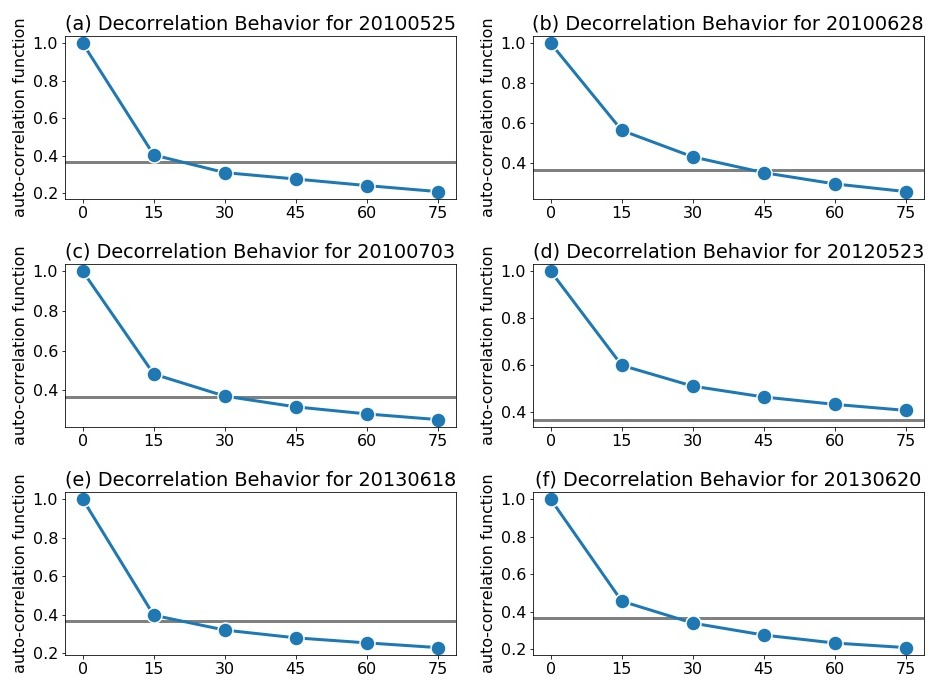
\includegraphics[width=\textwidth]{Grafiken/Abbildungen/decorrelation_CI.jpg}
\caption{Decorrelation analysis of the CI field for different case days from (a) to (f). Time-lagged pattern correlation coefficients have been calculated and averaged for one day. Grey line is at $\exp[-1]$ which marks the e-folding value. }
\label{fig:decorr_analysis}
\end{figure}

In a second exercise, we count how long each pixel is occupied by subsequent CI detections. This can be converted into a probability that a CI detection lives longer than a specified time interval. The results of this analysis are shown in Fig.~\ref{fig:life-time} for the low probability category $>25\%$. The figure shows that a relatively small fraction of the CI detection exhibits persistence. The probability for CI detections to live longer than 15~min lies between 10 and 20\%. Only a few percent of the CI detection live longer than 30~min.

\begin{figure}
\centering
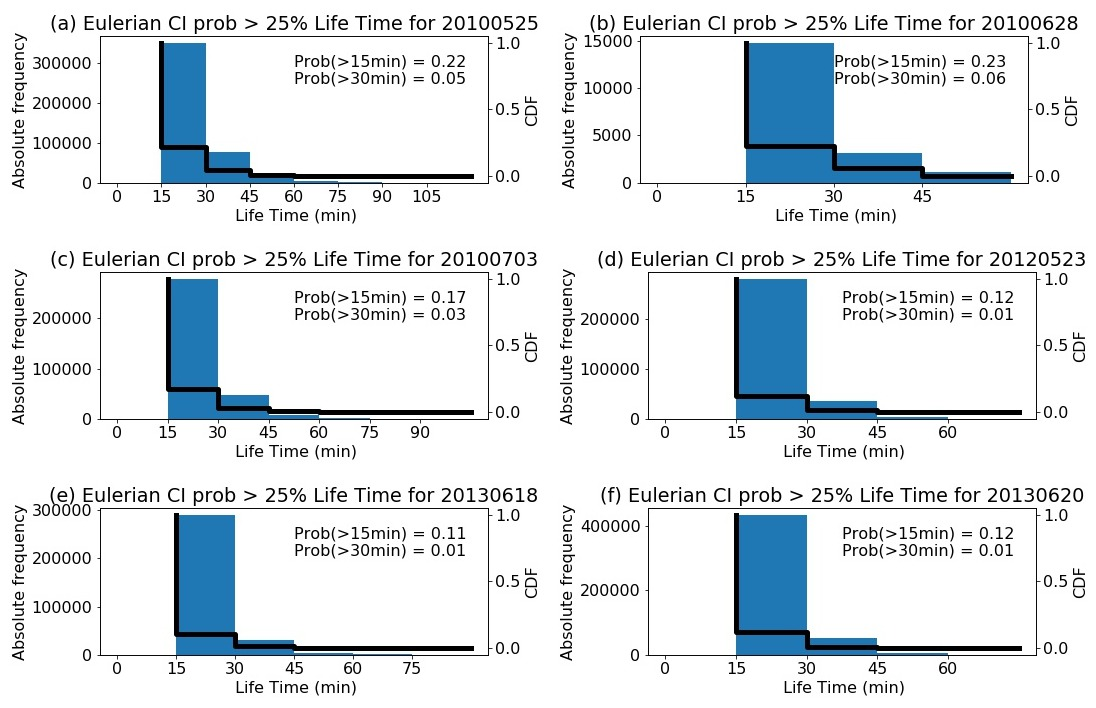
\includegraphics[width=\textwidth]{Grafiken/Abbildungen/life_time_CI25.jpg}
\caption{Eulerian life-time analysis of CI pixels in the category $>25\%$ for the different cases days.  Absolute frequencies of different life times are shown with blue bars, the probability that CI live longer than a certain time interval is given with black solid lines. }
\label{fig:life-time}
\end{figure}

For the higher probability CI categories, the situation is different: nearly all CI detections for and $>75\%$ live only one time step. These detection show no persistence. Thus, the de-correlation behaviour of the CI fields is dominated by the persistent character of the low probability CI events. Again, we recognise a very different behaviour of the low vs. high probability CI fields.

\section{Dominant cloud type of CI detections}
Another question inspired by the provided cloud and precipitation movies is which cloud type the CI detections have. Optimally, the CI detections should not be located in regions where there is no cloud or over cirrus clouds as cirrus cases are known to be problematic for CI detection algorithms . To analyse this, the NWC\,SAF v2013 cloud types of all CI detection pixels where collected for the 23\textsuperscript{rd} May 2012. 

As to be seen in Fig.~\ref{fig:ci_cloud_type}, the majority of CI pixels have expected cloud types .  More than \SI{90}{\percent} of the CI detections have a cloud type of very low, low and medium level clouds and fractional clouds, which makes sense. But there is also a small fraction having a cloud type of semi-transparent very thin clouds, which are cirrus clouds, and there is also a fraction of CI detections located over cloud free pixels.

Looking at the diurnal variation in the cloud type of CI detections Fig.~\ref{fig:ci_cloud_type_time}, it it becomes clear that the problem of CI detections with unexpected cloud types is linked to night times.  A likely explanation are differences in the version 2013 of the cloud type product used by TROPOS for this analysis and the version 2016 used by Meteo France for generating the CI product. Another possible option is, that there is a difference between the versions 2013, used in this analysis, and 2016, used for the CI product, of the NWC\,SAF cloud type product, especially in night time. But as this problem mainly effects the time span outside of the time frame used for the analyses of this study, no further investigation of this problem was conducted. 

\begin{figure}
\centering
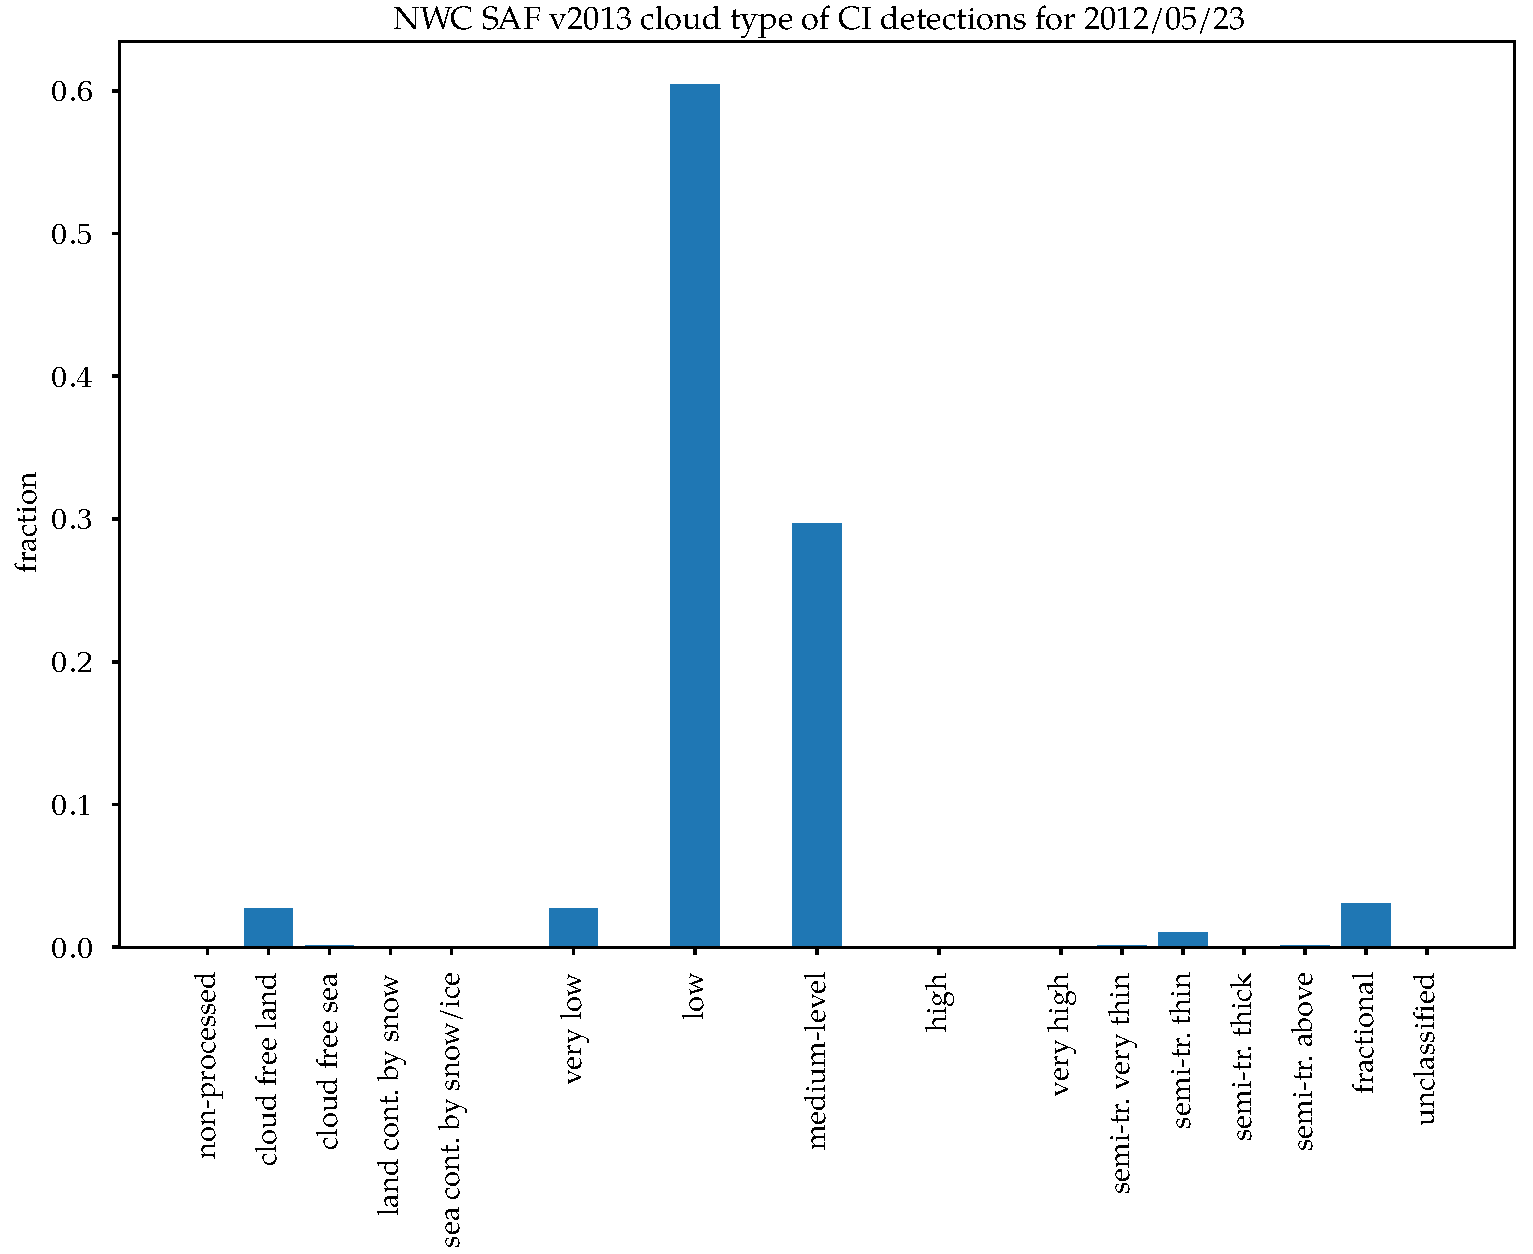
\includegraphics[width=0.9\textwidth]{Grafiken/Abbildungen/ci_cloud_types.pdf}
\caption{NWC\,SAF v2013 cloud types of CI detection pixels for 2012/05/23.}
\label{fig:ci_cloud_type}
\end{figure}

\begin{figure}
\centering
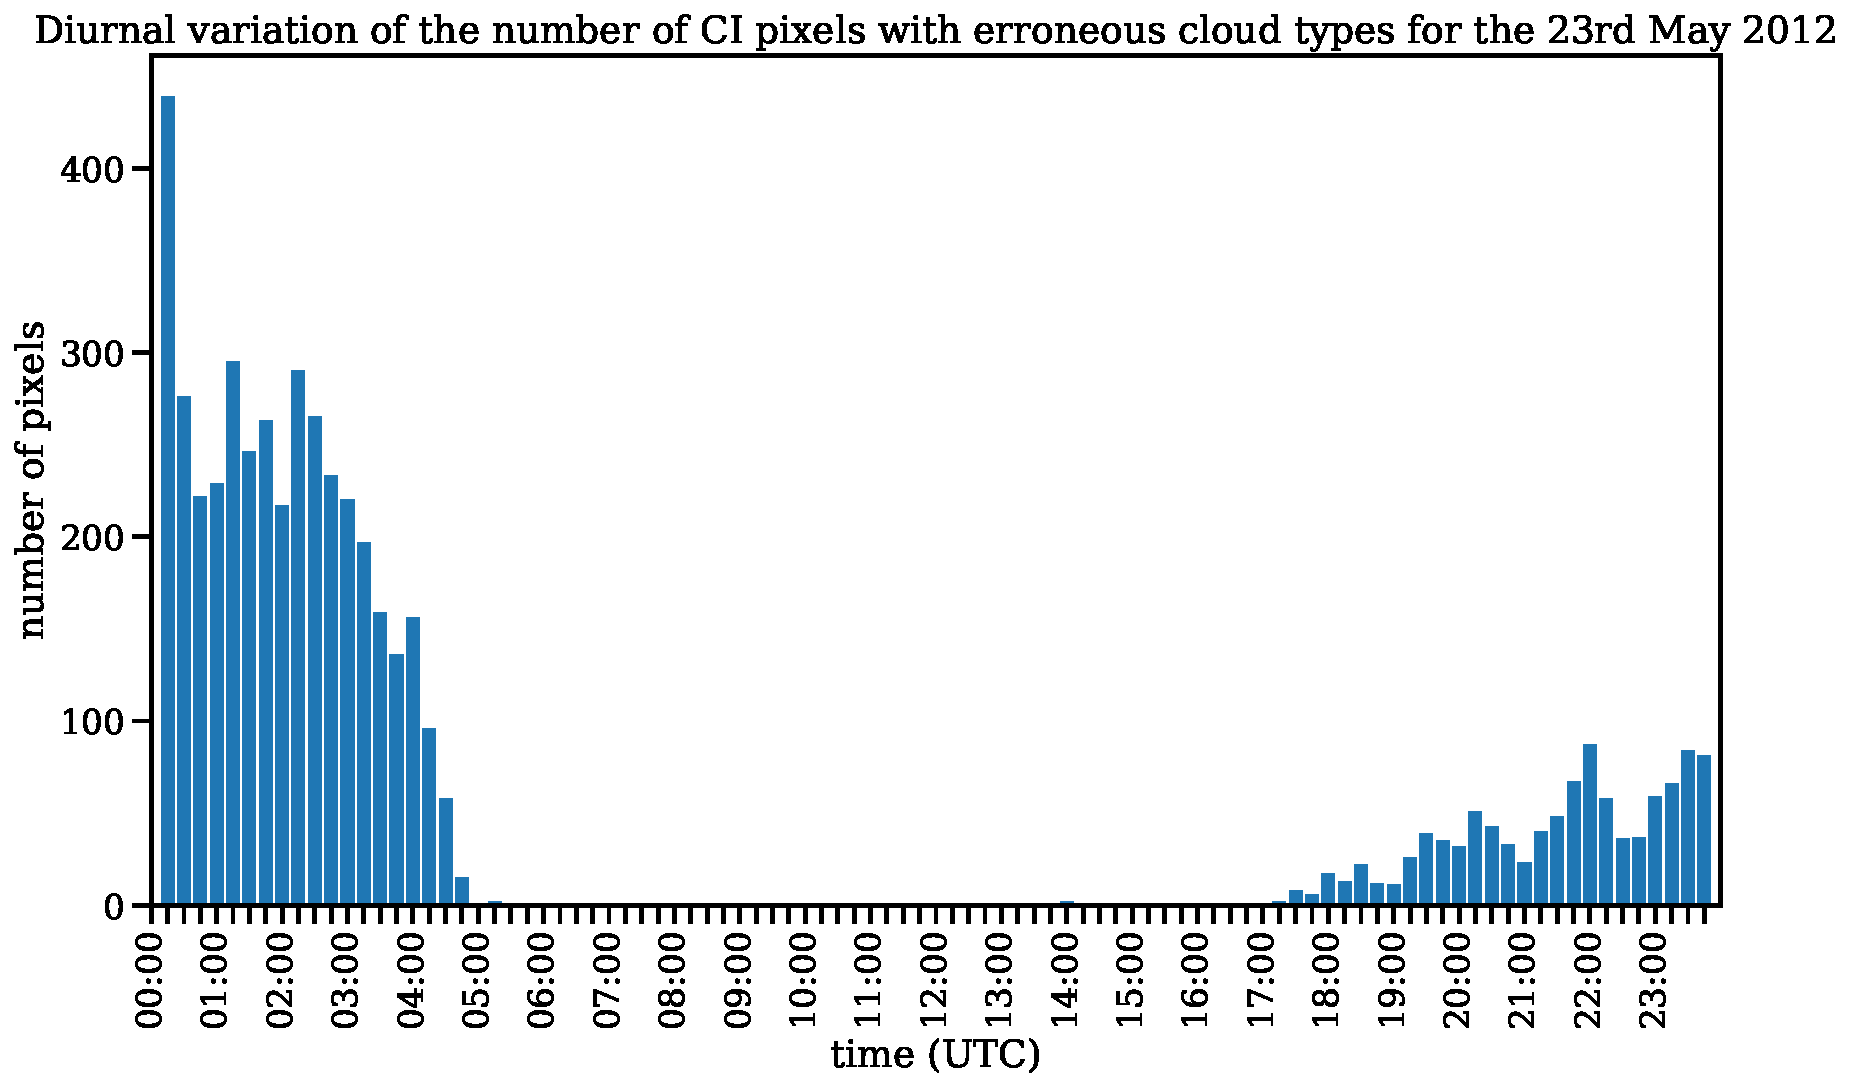
\includegraphics[width=0.8\textwidth]{Grafiken/Abbildungen/ci_cloud_types_time.pdf}
\caption{Diurnal variation of the number of CI detection pixels with erroneous cloud types for the 23\textsuperscript{rd} May 2012.}
\label{fig:ci_cloud_type_time}
\end{figure}